\chapter{Implementation and analysis} 
\label{chap:4}
\noindent In the previous chapter, we mainly identified several subsets of cross-ledger communication schemes and explained the related projects in details. Nevertheless, clear logic levels do not necessarily ensure a good user experience or functional applications. Thus, to evaluate the performance of different protocols or platforms, it is necessary to design and implement appropriate approaches. \\
\noindent As we discussed in section~\ref{sec:sol}, to realize cross-chain communication 

\section{HTLC Atomic-swaps implementation}
\noindent 
\newpage
\begin{figure}[H]
	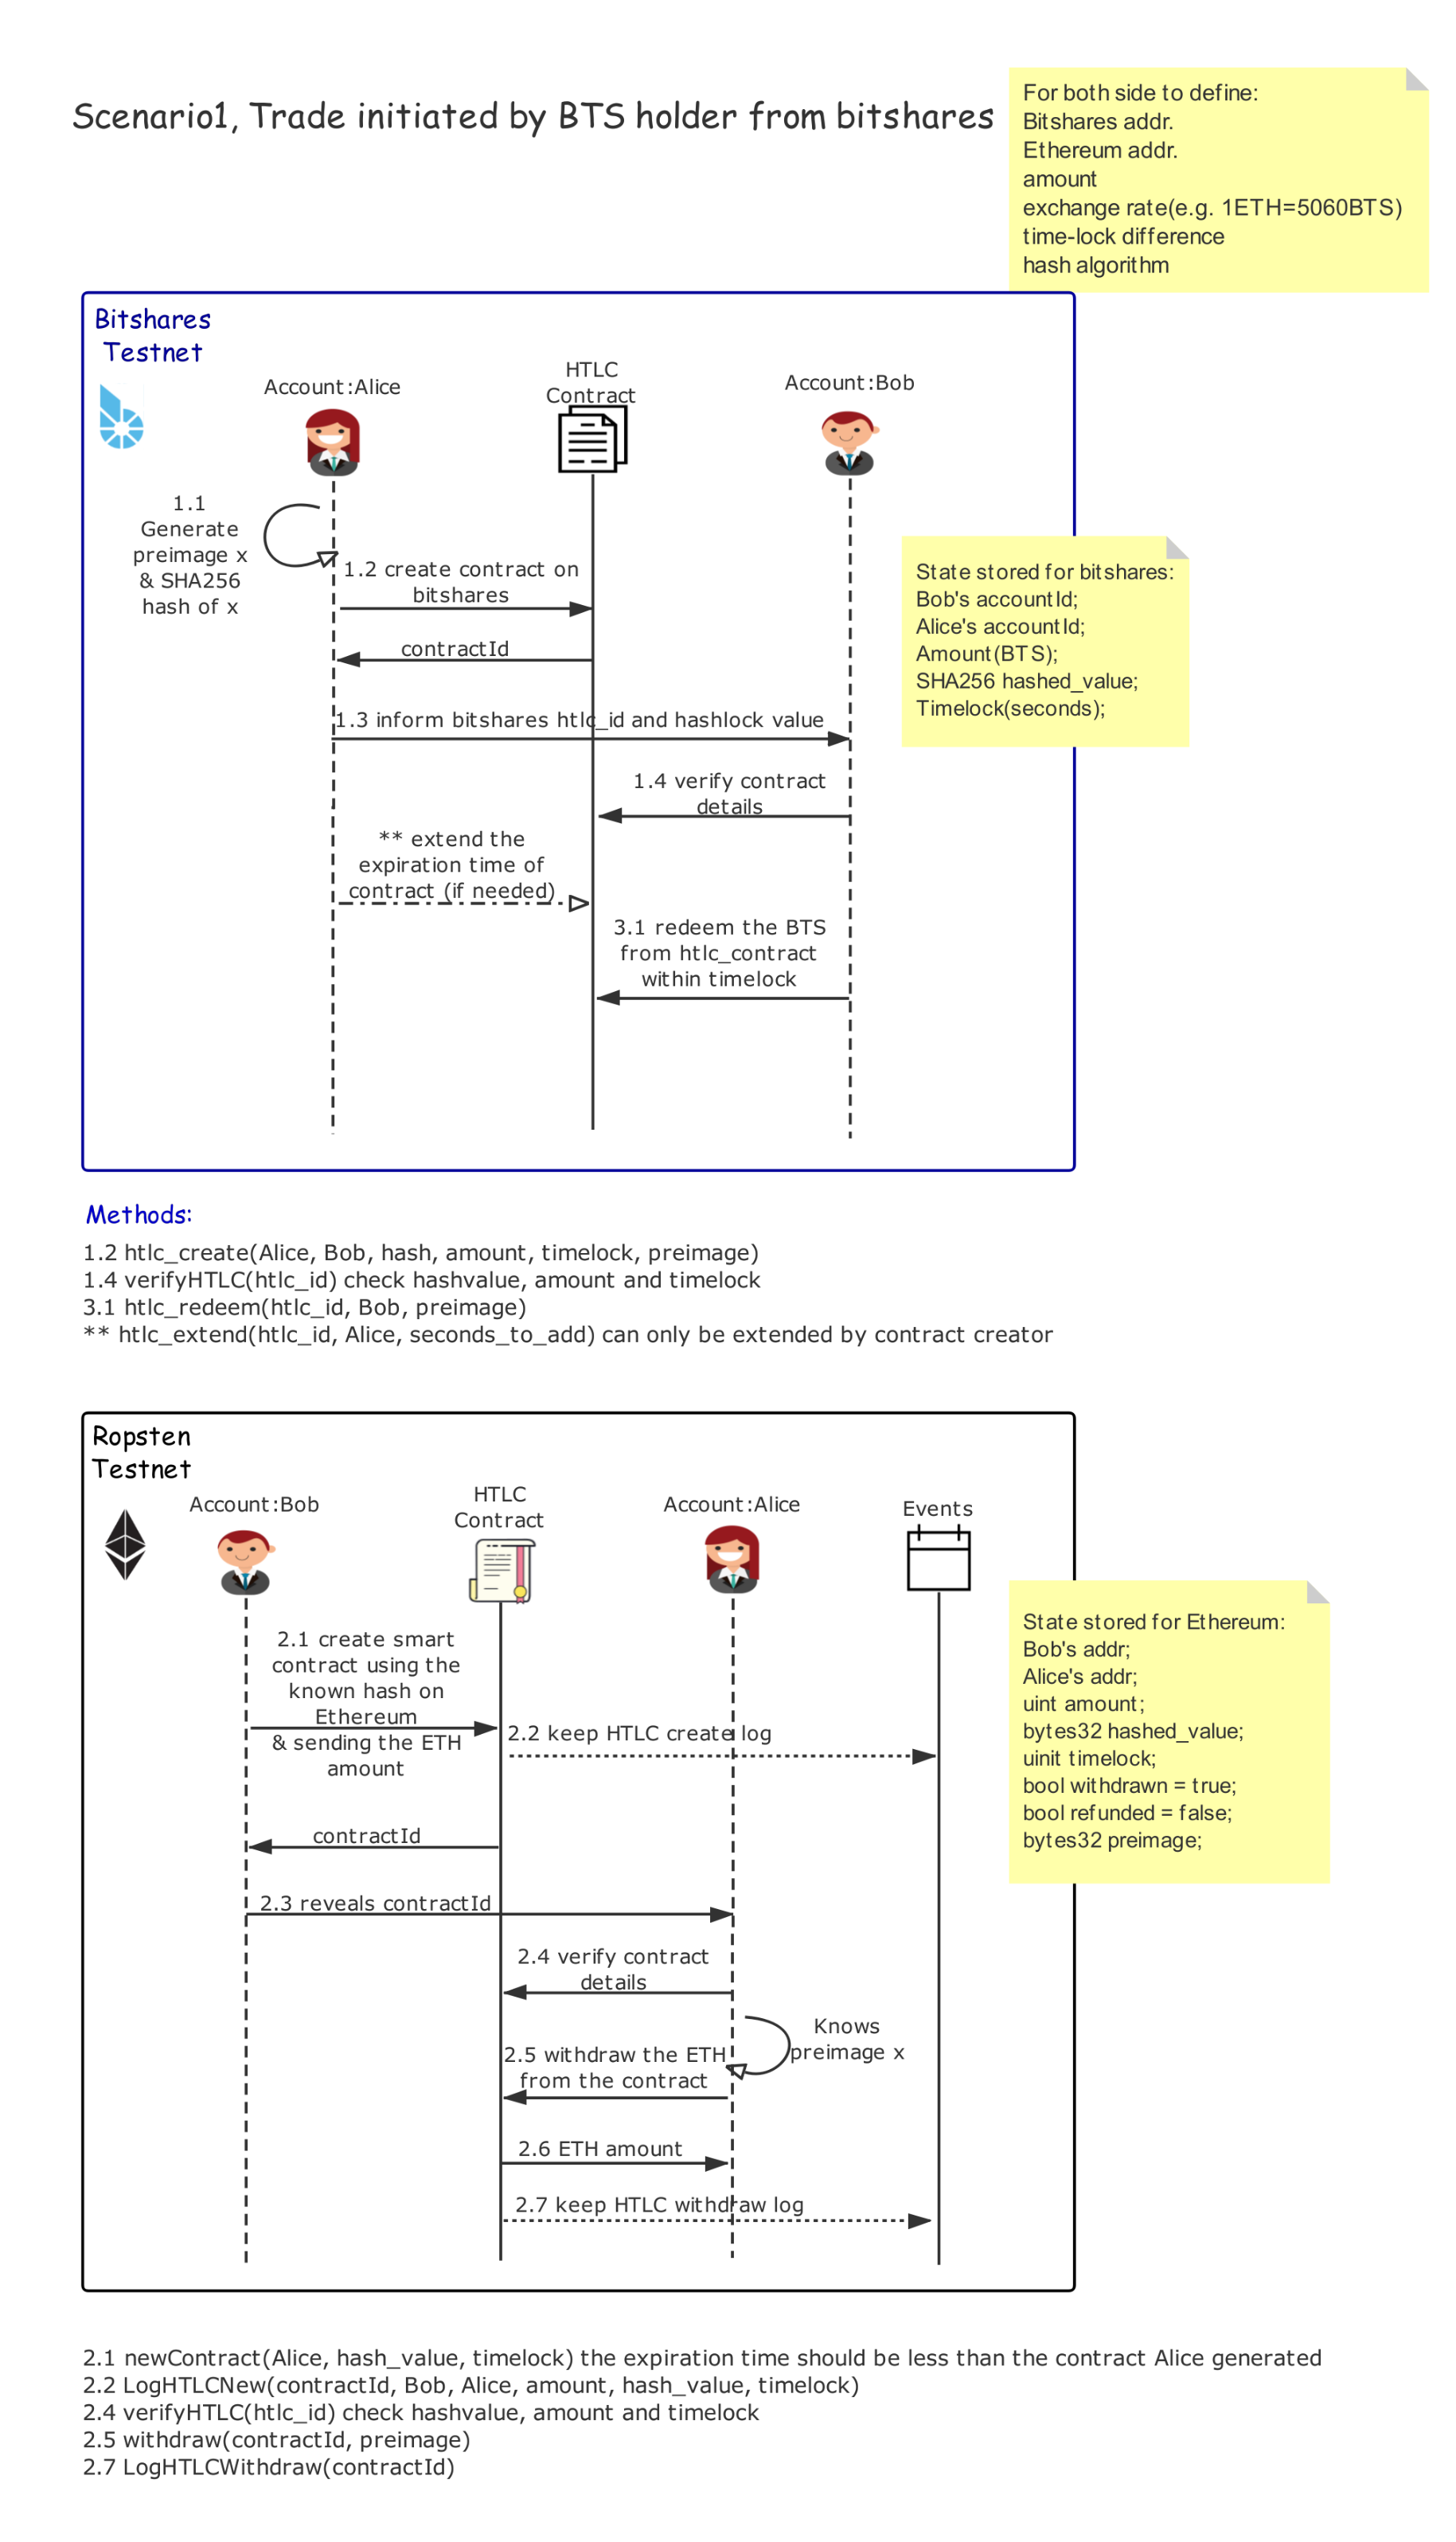
\includegraphics[width=1\textwidth]{./figures/BTS-ETH_diagram}
        \centering
        \caption{BTS->ETH swap diagram}
        \centering
        \label{fig:success}

\end{figure}
\begin{figure}[H]
	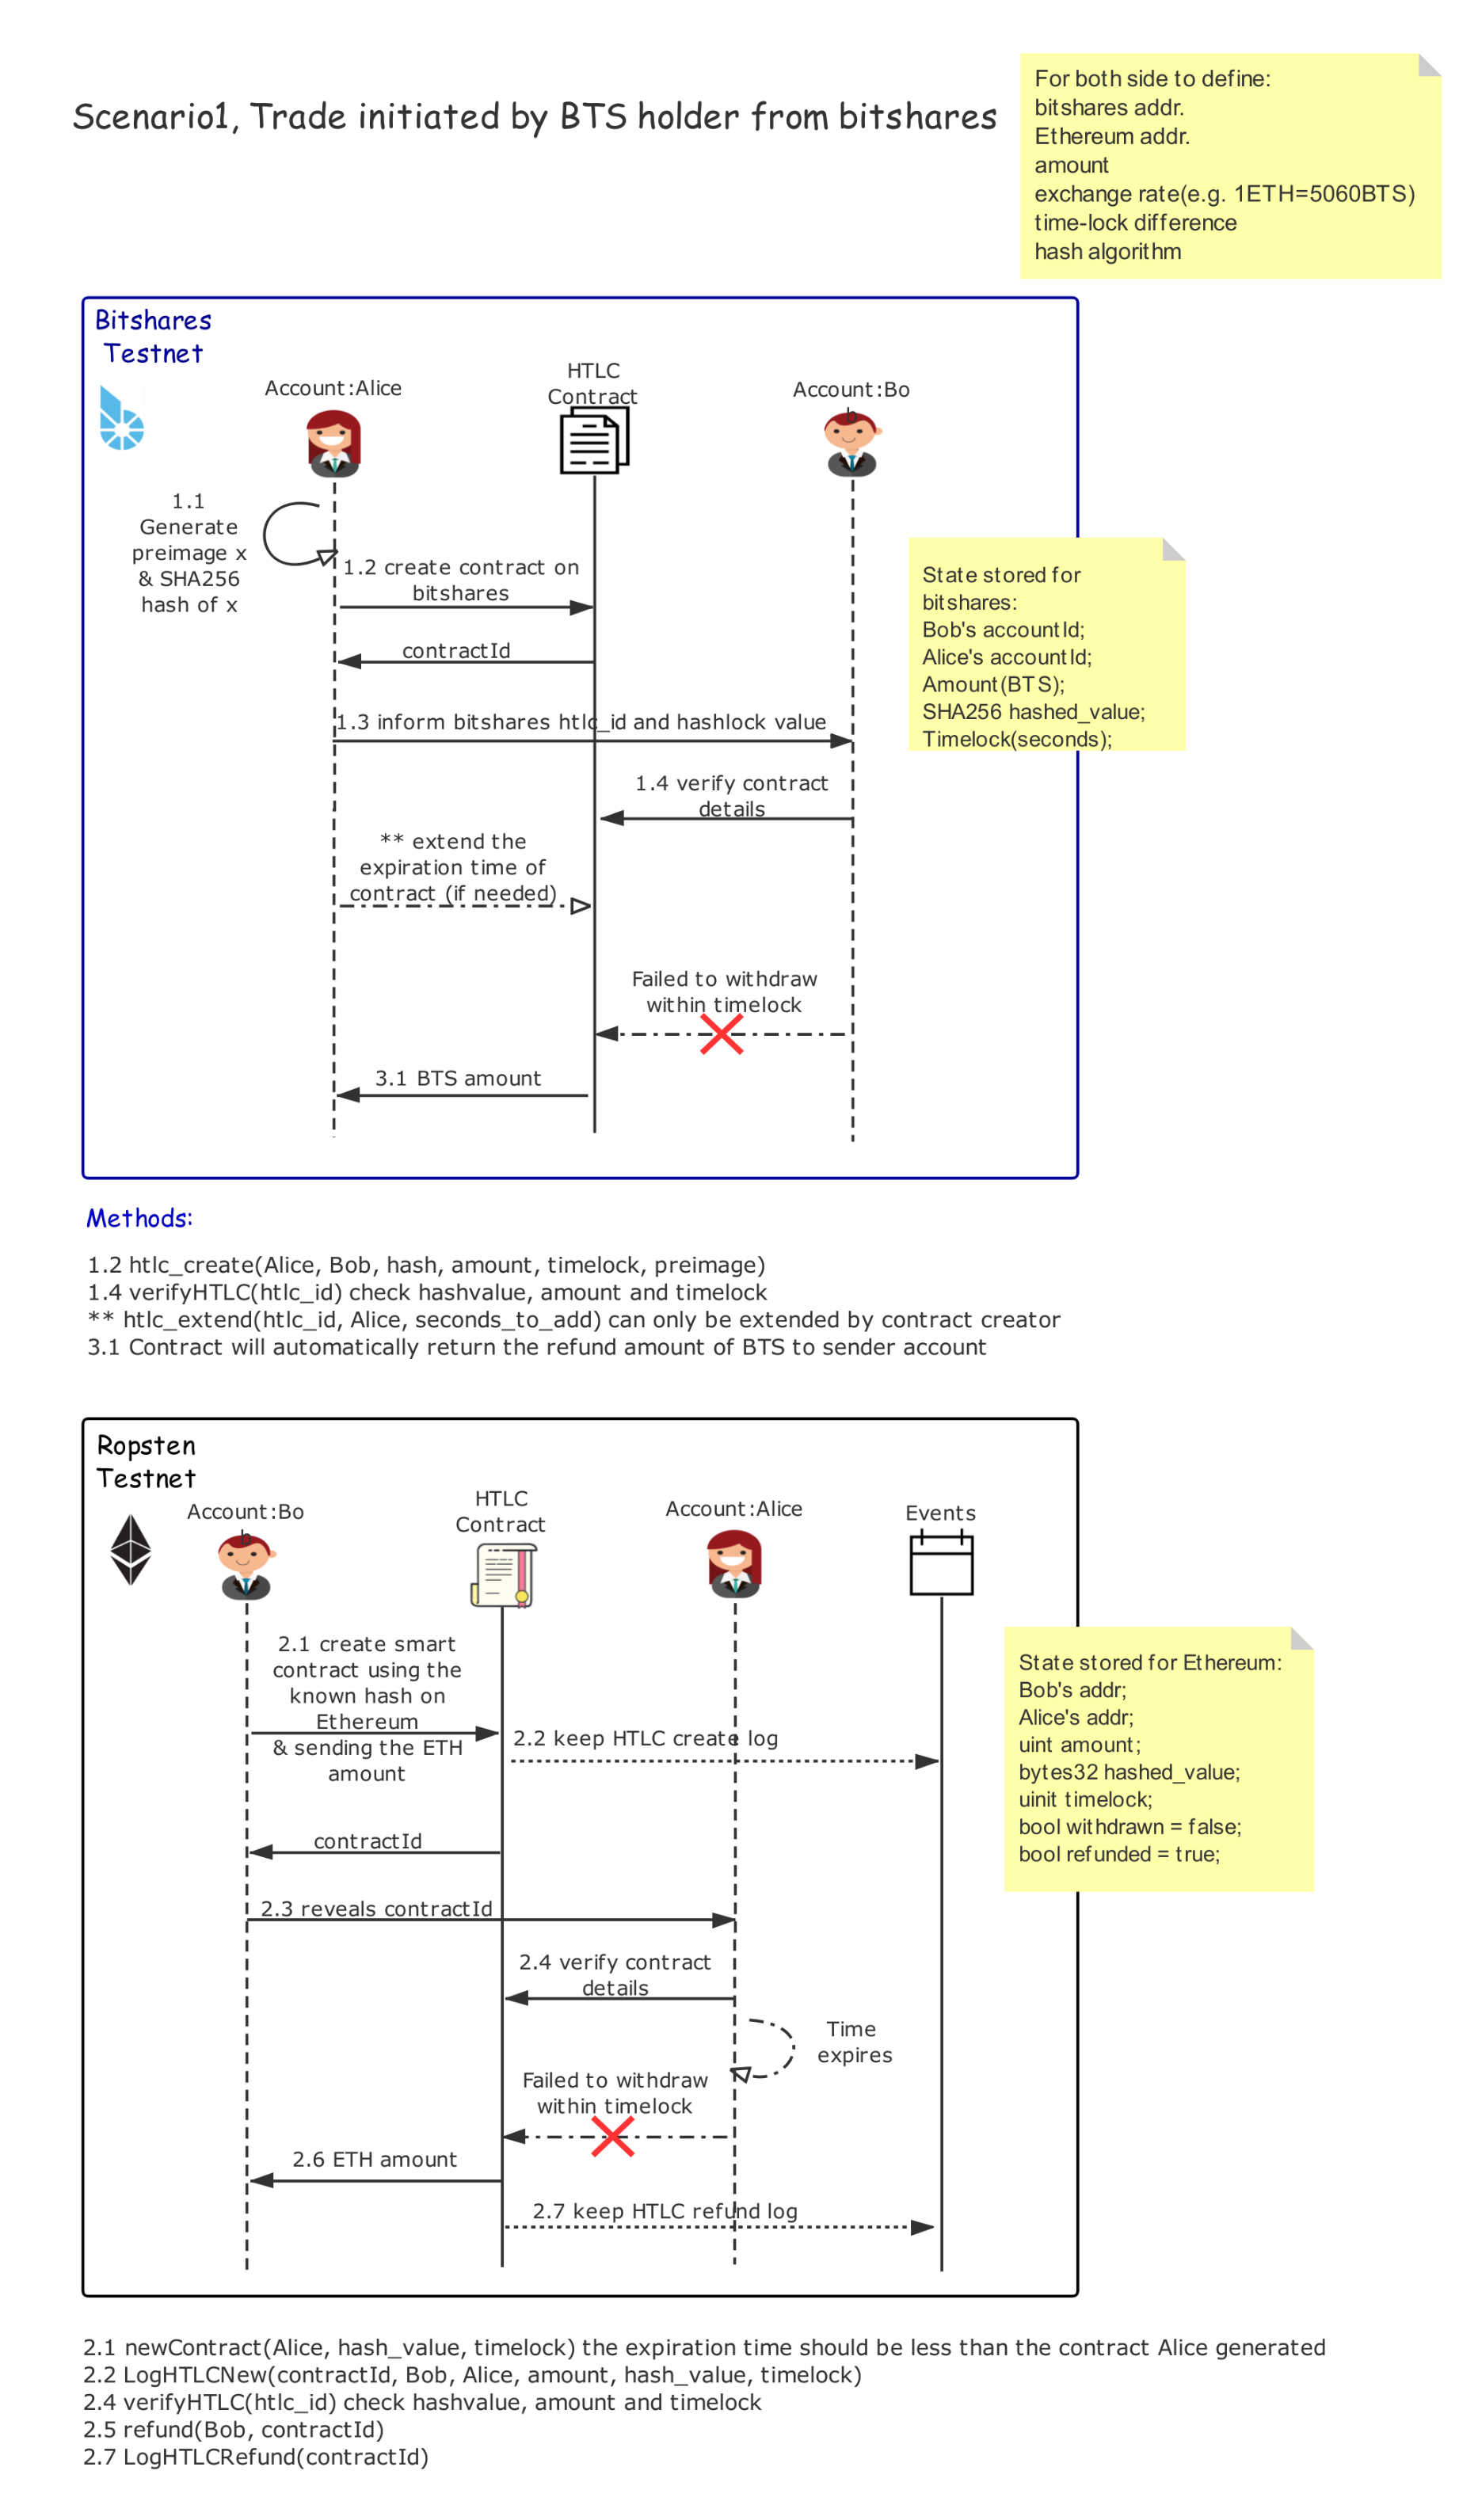
\includegraphics[width=1\textwidth]{./figures/BTS-ETH_diagram_failed}
        \centering
        \caption{BTS->ETH swap diagram}
        \centering
        \label{fig:failed}

\end{figure}


\section{Interledger switch API study}
\begin{figure}[H]
	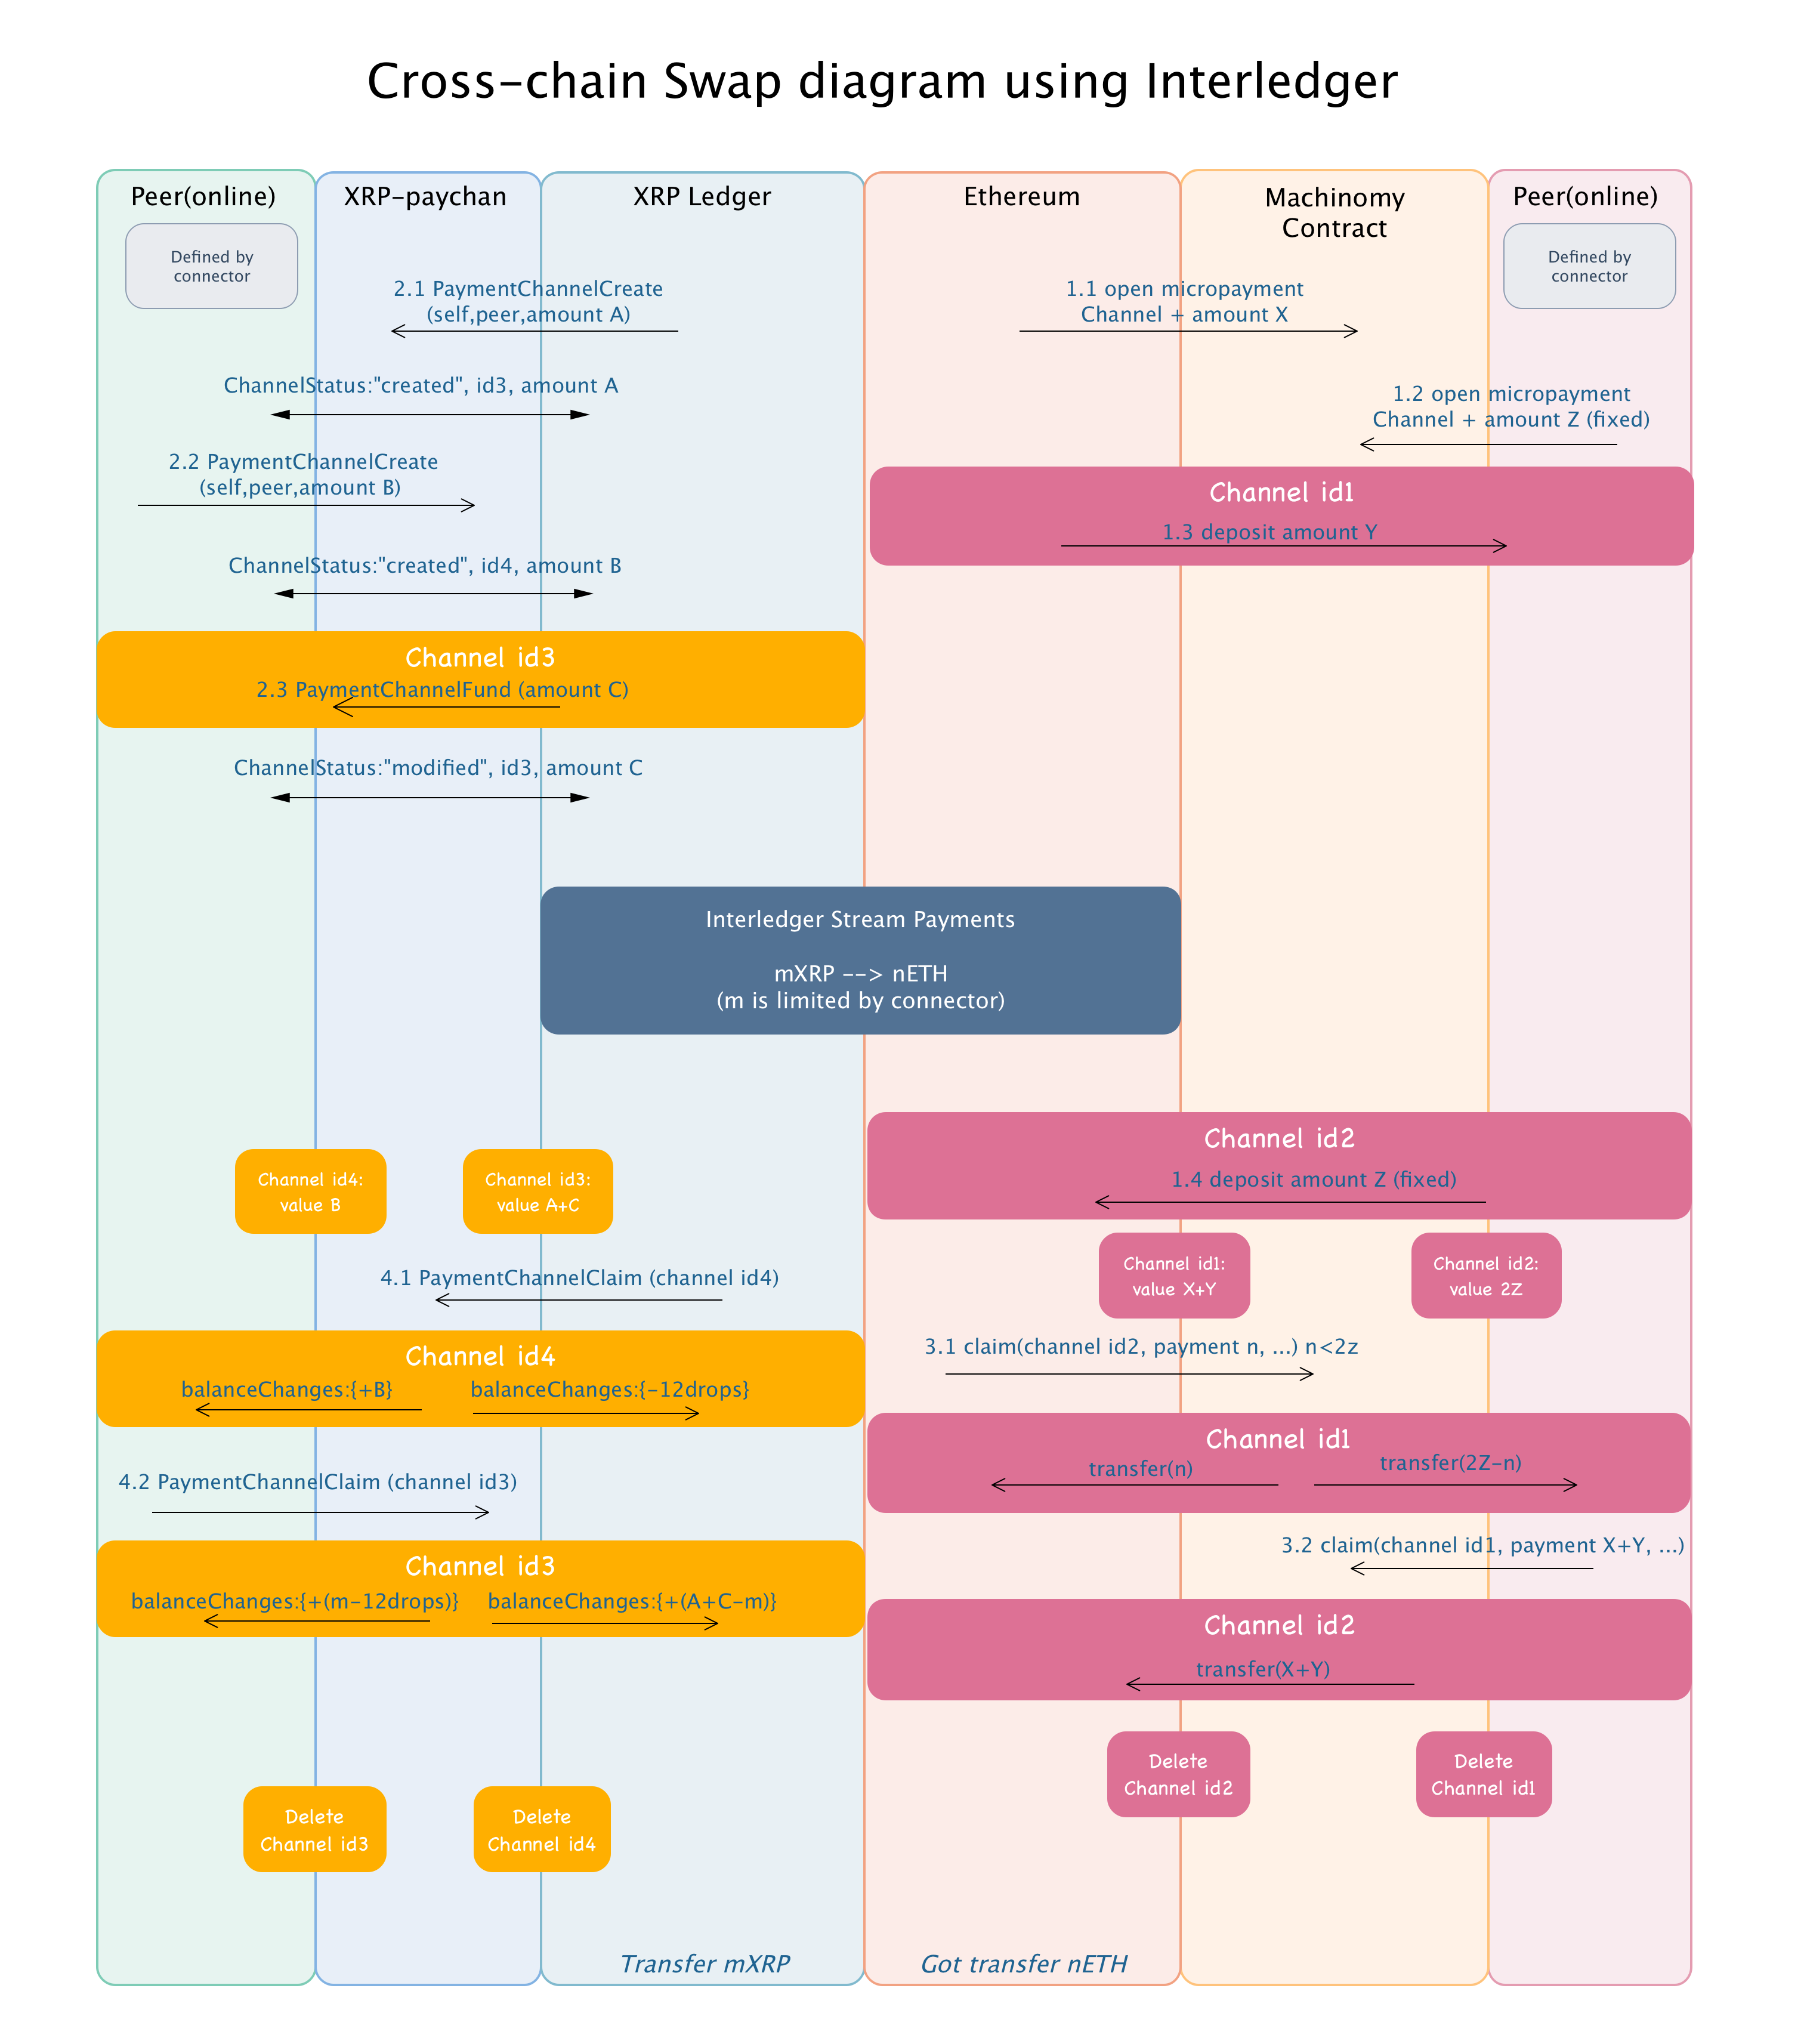
\includegraphics[width=1.5\textwidth]{./figures/XRP->ETH}
        \centering
        \caption{XRP->ETH}
        \centering
        \label{fig:xtoe}

\end{figure}
\begin{figure}[H]
	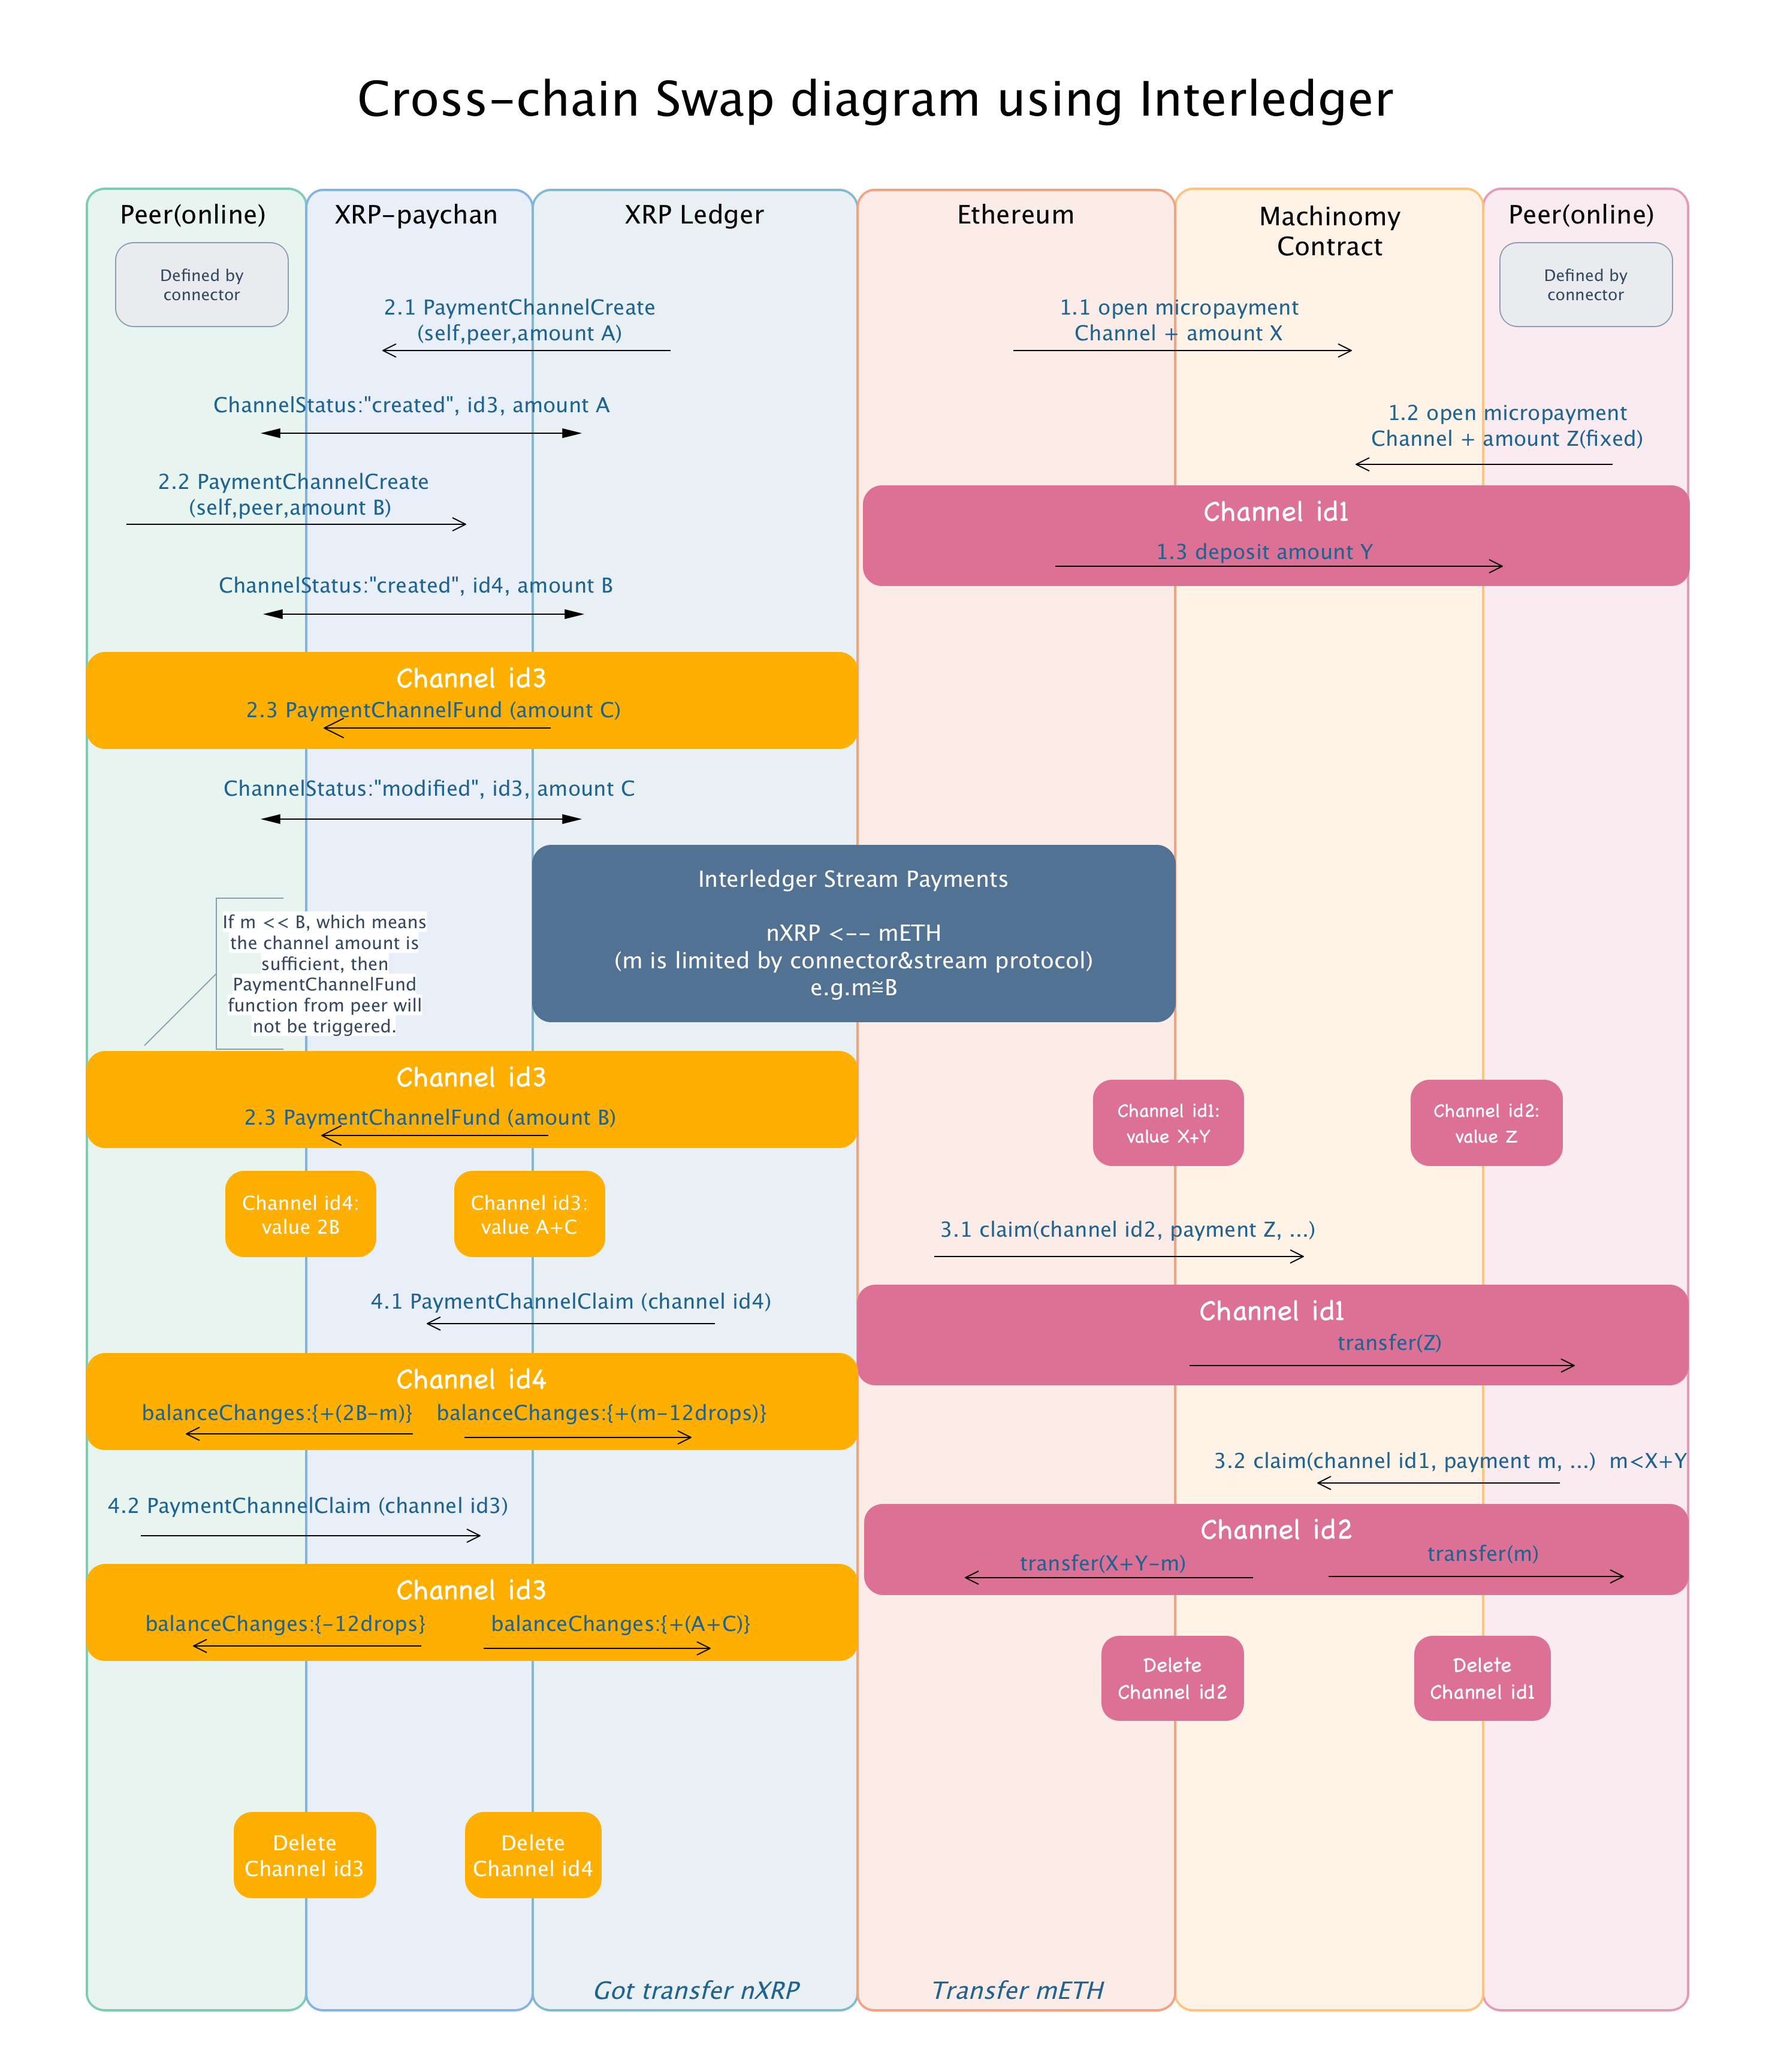
\includegraphics[width=1\textwidth]{./figures/ETH->XRP}
        \centering
        \caption{}
        \centering
        \label{fig:etox}

\end{figure}
\section{Summary}

Write here...
